\section{Analyse des Schmalbandinterferogramms}
Der Wellenl�ngenbereich des Muffelofen wird mit einem Schmalbandfilter reduziert. Da durch die Filterung auch die Intensit�t verringert wird, muss die Verst�rkung des Log-In-Verst�rkers korrigiert werden. Aufgrund des Filters wird eine ged�mpfte Cosinus-Schwingung symmetrisch um den Wei�lichtpunkt des Muffelofen erwartet. Aus dem aufgenommen Interferogramm soll die Wellenl�nge der maximalen Transmission und die Breite des 1/e-Abfalls der Einh�llenden bestimmt werden. Mit diesen beiden Werten kann die Breite des Schmalbandfilters bestimmt werden.
Das Interferogramm ist in Abbildung \ref{fig:filter_weiss} zu sehen. 

\begin{figure}[H]
\centering
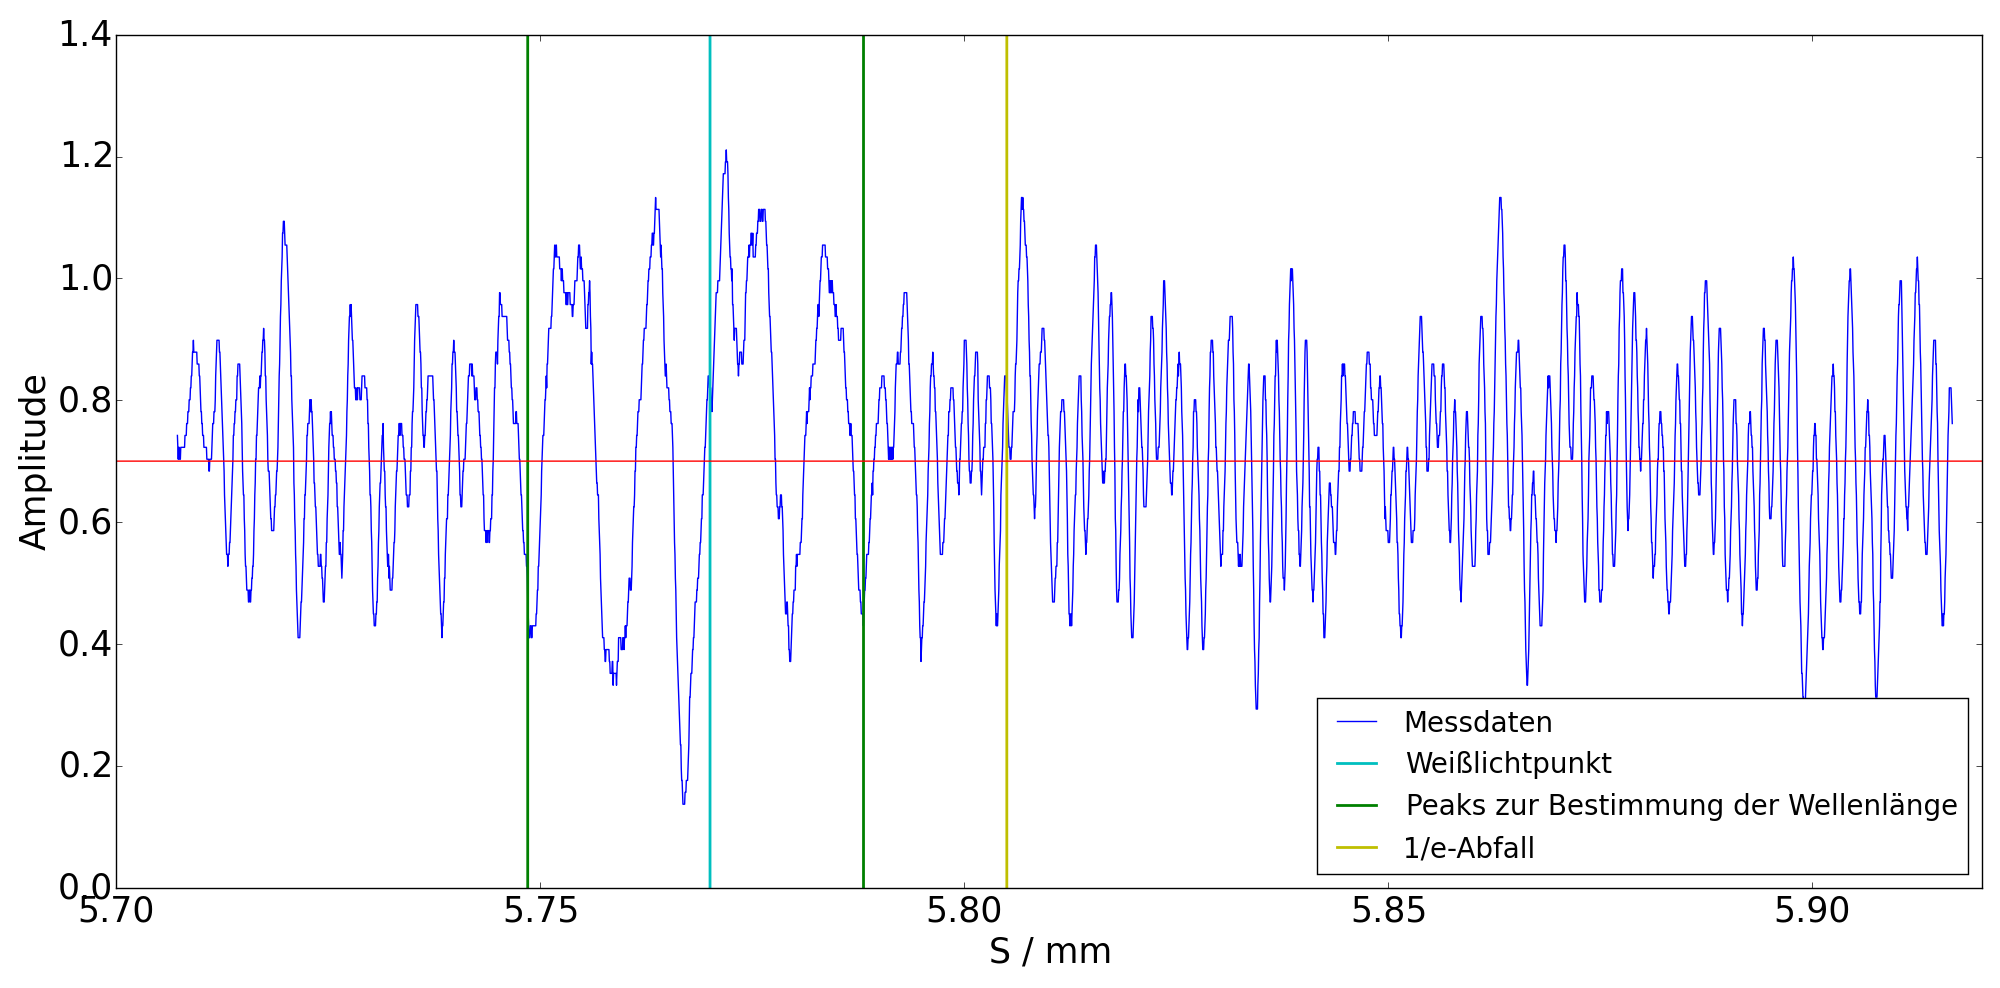
\includegraphics[scale = 0.33]{filter_weiss.png}
\caption{Interferogramm f�r den Muffelofen mit Schmalbandfilter. Die gr�nen Linien markieren den Bereich f�r die Bestimmung der Wellenl�nge, die rote Linie markiert die Nulllage}
\label{fig:filter_weiss}
\end{figure}

Aus den Interferrogramm ergeben sich die Werte in Tabelle ??. Es wurde ein kleines Intervall um den Wei�lichtpunkt gew�hlt, da in diesem Bereich die Abst�nde zwischen den Peaks regelm��ig sind.

\begin{table}
\centering
\caption{Messwerte f�r die Bestimmung der Wellenl�nge des Wei�lichtpunkts}
\label{tab:parameter_filter}
\end{table}